A partir dos controladores de atitude e altitude fuzzy projetados, foram propostos dois controladores do tipo neuro-fuzzy: um para cada dos casos.

Para tanto, foram utilizados os códigos mostrados nos Apêndices \ref{chap:train-anfis-altitude} e \ref{chap:train-anfis-atitude}. No processo de criação do controlador de altitude neuro-fuzzy, foram gerados trezentos\footnote{Este valor foi arbitrado por corresponder a uma quantidade razoável para treinar a RNA sem que se alcance o sobreajuste, conhecido como \textit{overfitting}} pares de entradas e cada um deles foi submetido ao processo de inferência fuzzy utilizando o controlador previamente modelado. Dois terços desses dados foram utilizados para gerar o conjunto de treinamento, representado pela variável {\ttfamily train} e o um terço restante foi armazenado na variável {\ttfamily test} e utilizado para validação do treinamento. Então, utilizando o comando {\ttfamily mam2sug} do MATLAB, foi gerado um modelo fuzzy Sugeno a partir do Mamdani que havia sido modelado e este novo arquivo foi salvo sob o nome {\ttfamily fis\_altitude\_neuro.fis}.

Feito isto, utilizou-se o comando comando {\ttfamily anfisedit} para abrir o \textit{Neuro-Fuzzy Designer} do MATLAB, cuja interface é mostrada na Figura \ref{fig:anfisedit_screen}. No campo marcado pelo número 2 na imagem (\textit{Generate FIS}), clicou-se no botão \textit{Load} e se selecionou o arquivo {\ttfamily fis\_altitude\_neuro.fis} que fora gerado pelo código executado. Após isto, no campo marcado pelo número 1 (\textit{Load Data}), marcou-se \textit{Training} e \textit{worksp} para utilizar uma variável da área de trabalho do MATLAB para treinar a rede. Após clicar em \textit{Load Data}, digitou-se {\ttfamily train}, nome da variável definida no código. Então, no campo marcado pelo número 3, marcou-se \textit{Training Data} e se clicou no botão \textit{Test Now} para executar o treinamento da rede. Após estes passos, a rede neuro-fuzzy foi devidamente treinada e sua estrutura, mostrada na Figura \ref{fig:rna_anfis_altitude_gray}, pode ser obtida clicando no botão \textit{Structure} logo acima do campo 3. Esta estrutura relaciona as variáveis de entrada e suas funções de pertinência, através das regras fuzzy, à saída do sistema e às suas funções de pertinência, em que cada componente representa um neurônio da RNA obtida. 

\begin{figure}[!htb]
    \centering
    \caption{Interface gráfica da ferramenta \textit{Neuro-Fuzzy Designer} com destaque aos três campos necessários para treinamento e teste da rede neuro-fuzzy}
    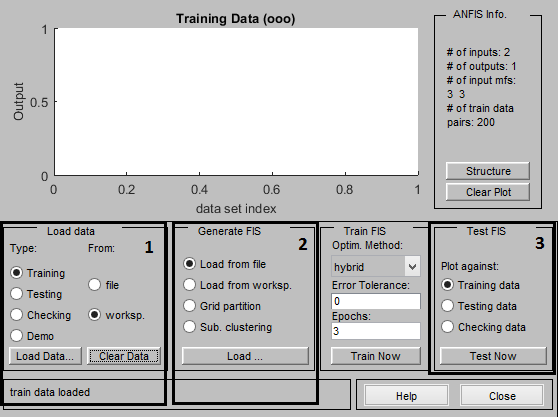
\includegraphics[width=0.8\textwidth]{./04-figuras/anfisedit/anfisedit_screen}
    \label{fig:anfisedit_screen}
\end{figure}

\begin{figure}[!htb]
    \centering
    \caption{Diagrama da RNA referente ao controlador neuro-fuzzy para altitude}
    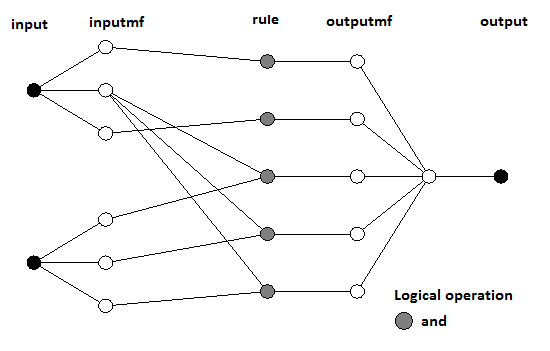
\includegraphics[width=0.6\textwidth]{./04-figuras/anfisedit/rna_anfis_altitude_gray}
    \label{fig:rna_anfis_altitude_gray}
\end{figure}

Após o término do treinamento, deve-se submeter a rede ao processo de treinamento. Para tanto, basta selecionar \textit{Testing} no campo marcado pelo número 1, deixar marcada a opção \textit{worksp}, clicar no botão \textit{Load Data} e escolher a variável {\ttfamily test}, que também foi definida no código executado.

A Figura \ref{fig:rna_anfis_train_result_altitude} mostra o gráfico obtido na ferramenta após o processo de treinamento, em que os círculos brancos mostram os dados utilizados no treinamento e os asteriscos pretos indicam o valor referentes a eles obtidos pela rede treinada.

\begin{figure}[!htb]
    \centering
    \caption{Resultado obtido pelo treinamento da RNA para controle de altitude}
    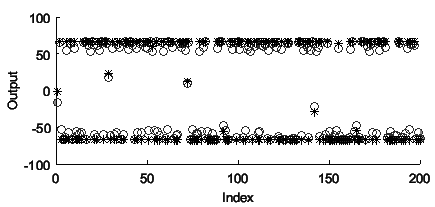
\includegraphics[width=0.6\textwidth]{./04-figuras/anfisedit/rna_anfis_train_result_altitude}
    \label{fig:rna_anfis_train_result_altitude}
\end{figure}

%Feito isto, após utilizar o comando {\ttfamily anfisedit} para abrir o \textit{Neuro-Fuzzy Designer} do MATLAB, carregou-se, nesta ferramenta, o arquivo {\ttfamily fis\_altitude\_neuro.fis} como sistema a ser treinado e, utilizando as variáveis {\ttfamily train} e {\ttfamily test}, o sistema foi devidamente treinado e validado. Após este processo, obteve-se um controlador neuro-fuzzy cujo funcionamento é mostrado pela superfície de regras mostradas na Figura \ref{fig:u1_sugeno_surface}.

Um processo similar foi aplicado para modelar o controlador de atitude neuro-fuzzy, como mostra o Apêndice \ref{chap:train-anfis-atitude}. As Figuras \ref{fig:rna_anfis_atitude_gray} e \ref{fig:rna_anfis_train_result_atitude} mostram o diagrama da RNA referente ao controlador neuro-fuzzy para atitude e o resultado obtido pelo seu treinamento respectivamente.

\begin{figure}[!htb]
    \centering
    \caption{Diagrama da RNA referente ao controlador neuro-fuzzy para atitude}
    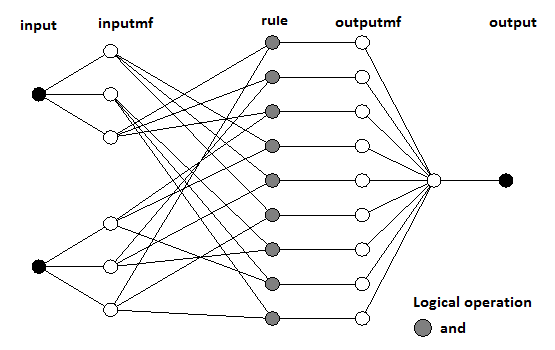
\includegraphics[width=0.6\textwidth]{./04-figuras/anfisedit/rna_anfis_atitude_gray}
    \label{fig:rna_anfis_atitude_gray}
\end{figure}

\begin{figure}[!htb]
    \centering
    \caption{Resultado obtido pelo treinamento da RNA para controle de atitude}
    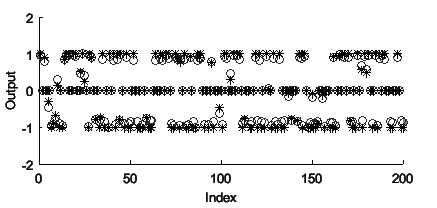
\includegraphics[width=0.6\textwidth]{./04-figuras/anfisedit/rna_anfis_train_result_atitude}
    \label{fig:rna_anfis_train_result_atitude}
\end{figure}

O processo de treinamento determina o comportamento dos controladores neuro-fuzzy projetados, cujas superfícies de regras são exibidas nas Figuras \ref{fig:u1_sugeno_surface} e \ref{fig:u2_u3_sugeno_surface}.

%-----
%Utilizando o comando {\ttfamily mam2sug} do MATLAB, obteve-se um novo modelo fuzzy do tipo Sugeno para cada modelo previamente definidos: um para controle de altitude e um segundo para controle de atitude do quadrotor. Então, utilizando o \textit{Neuro-Fuzzy Designer} do MATLAB, cada um dos modelos Sugeno criados foi treinado a partir de resultados obtidos pelos modelos fuzzy previamente elaborados. Não houve nenhuma alteração nas regras dos sistema, mas, devido às generalizações e aprendizagem da rede neuro-fuzzy, a relação entre valores de cada conjunto de saída foi ligeiramente alterado. Isso pode ser visto a partir das superfícies de regras para ambos os controladores, mostradas nas Figuras \ref{fig:u1_sugeno_surface} e \ref{fig:u2_u3_sugeno_surface}.

% Mostrar superfície Sugeno
\begin{figure}[!htb]
    \centering
    \caption{Superfície das regras do sistema de controle neuro-fuzzy para a altitude do quadrotor}
    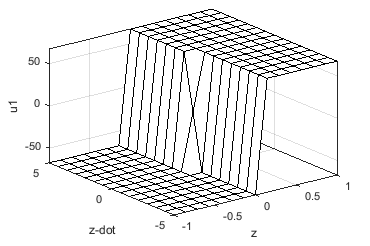
\includegraphics[width=0.6\textwidth]{./04-figuras/resultados/fis_u1/u1_sugeno_surface}
    \label{fig:u1_sugeno_surface}
\end{figure}

\begin{figure}[!htb]
    \centering
    \caption{Superfície das regras do sistema de controle fuzzy para a atitude do quadrotor}
    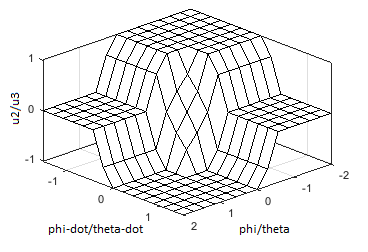
\includegraphics[width=0.6\textwidth]{./04-figuras/resultados/fis_u3/u2_u3_sugeno_surface}
    \label{fig:u2_u3_sugeno_surface}
\end{figure}


